\documentclass[11pt, a4paper]{article}
\usepackage[utf8]{inputenc}
\usepackage{geometry}
\geometry{margin=1in}
\usepackage{graphicx}
\usepackage{amsmath}
\usepackage{booktabs}
\usepackage{algorithm}
\usepackage{algpseudocode}
\usepackage{float} 

\title{Stage 6: Representations of an Operating System Process}
\author{Group Members}
\date{\today}

\begin{document}
\maketitle

\section*{Paragraph Representation of Idea}
An operating system (OS) acts as the foundational software layer that manages and controls all hardware and software components within a computer. Its startup sequence begins with a small program called a bootloader, which initializes the hardware and loads the core of the OS---the kernel---into main memory. Once activated, the kernel assumes full control of the system, efficiently allocating CPU time, managing memory processes, coordinating input/output devices, and providing a stable, secure environment where user applications can seamlessly execute.

\section*{Figure Representation of Idea}
\begin{figure}[H]
    \centering
    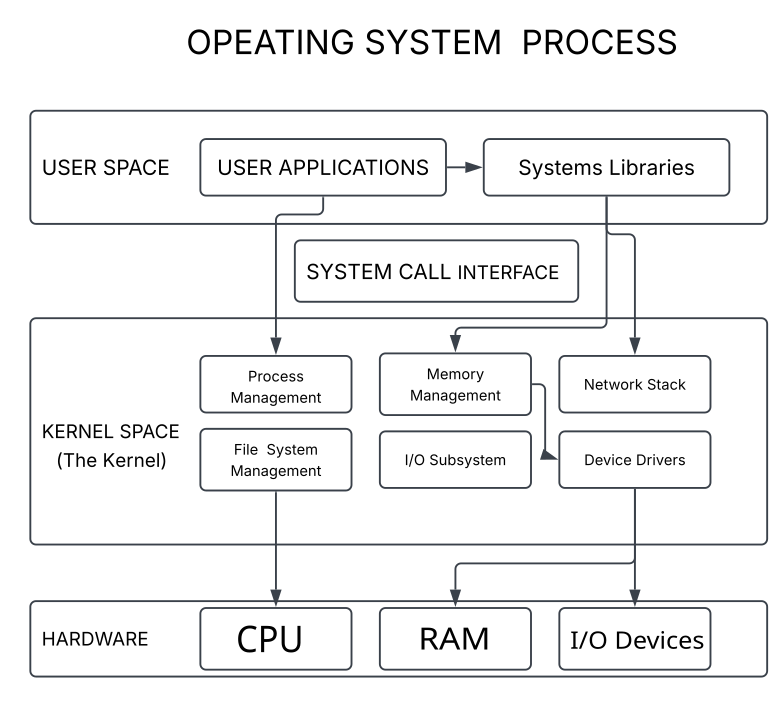
\includegraphics[width=0.9\textwidth]{os_process.png}
    \caption{Operating System Process}
    \label{fig:os_process}
\end{figure}

\section*{Table Representation of Idea}
\begin{table}[H]
    \centering
    \caption{System Component and Execution Phase}
    \label{tab:os_components}
    \renewcommand{\arraystretch}{1.4}
    \begin{tabular}{p{3.5cm} p{7cm} p{4cm}}
        \toprule
        \textbf{System Component} & \textbf{Primary Function} & \textbf{Execution Phase} \\
        \midrule
        Firmware (BIOS/UEFI) & Performs hardware checks (POST) and finds the boot device & Immediate Power-On \\
        Bootloader & Loads the kernel into main memory & Early Boot Sequence \\
        Kernel & Manages CPU, RAM, and hardware resource allocation & Continuous Operation \\
        Shell / User Space & Provides the interface for user applications to run & Post-Boot / Active \\
        \bottomrule
    \end{tabular}
\end{table}

\section*{Equation Representation of Idea}
\begin{equation}
    S_{t+1} = k \left( S_t, \sum_{i=1}^{h} I_i(t) + \sum_{j=1}^{s} C_j(t) \right) - \Delta_{overhead}
    \label{eq:os_state}
\end{equation}

\subsection*{Equation Breakdown}
\begin{itemize}
    \item \textbf{$S_{t+1}$ (Next System State):} The resulting state of the computer (e.g., updated memory allocation, next thread in the CPU, written data on the disk).
    \item \textbf{K (The Kernel Function):} The core operating system logic that processes inputs, enforces security, and allocates hardware resources.
    \item \textbf{$S_t$ (Current System State):} The exact configuration of the CPU registers, RAM, and I/O devices at the current moment in time.
    \item \textbf{$\Sigma I_{i(t)}$ (Hardware Interrupts):} The sum of all hardware signals happening at time t (e.g., a mouse click, a network packet arriving, a disk finishing a read).
    \item \textbf{$\Sigma C_{j(t)}$ (System Calls):} The sum of all software requests from user applications at time t (e.g., a browser asking for memory or attempting to write a file).
    \item \textbf{$\Delta_{\{overhead\}}$ (Context Switching Overhead):} The inevitable computational time and resources the OS consumes just to manage these transitions, representing the ``tax'' of running an OS.
\end{itemize}

\section*{Algorithmic Representation of Idea}

\begin{algorithm}[H]
\caption{OS Boot Sequence}
\begin{algorithmic}[1]
\State \textbf{START} OS\_Boot\_Sequence
\State Initialize CPU and apply power
\State Run Power-On Self Test (POST)
\If{hardware fails POST}
    \State HALT and display error code
\Else
    \State Identify primary boot device (SSD/HDD/Network)
    \State Load Bootloader from EFI System Partition / MBR
    \State Execute Bootloader
    \State Bootloader decompresses and loads Kernel into RAM
    \State Pass system control to Kernel
    \State Kernel initializes device drivers and memory structures
    \State Kernel mounts the root file system
    \State Kernel starts background system services (daemons)
    \State Launch Graphical User Interface (GUI) or Command Line Interface (CLI)
\EndIf
\State \textbf{END} OS\_Boot\_Sequence
\end{algorithmic}
\end{algorithm}

\section*{Bullet Point Representation of Idea}
The core responsibilities of an Operating System include:
\begin{itemize}
    \item \textbf{Process Management:} Creating, suspending, scheduling, and terminating software processes.
    \item \textbf{Memory Management:} Tracking available RAM and securely allocating it to active applications.
    \item \textbf{File System Management:} Organizing directories, writing data to storage, and enforcing file permissions.
    \item \textbf{Device Management:} Using drivers to facilitate seamless communication between the software and physical peripherals.
\end{itemize}

\section*{Numbered List Representation of Idea}
\begin{enumerate}
    \item The physical machine is powered on, sending a wake signal to the CPU.
    \item The motherboard firmware (BIOS/UEFI) executes a hardware diagnostic check.
    \item The firmware locates the bootable storage drive.
    \item The system executes the bootloader (such as GRUB or Windows Boot Manager).
    \item The bootloader transfers the core OS kernel into the system's memory.
    \item Kernel takes over hardware management, starts services, and presents the login screen to user.
\end{enumerate}

\end{document}